\documentclass[../main.tex]{subfiles}
\begin{document}

\subsection{Semantic Web}
\label{sec:semantic-web}

Einer der Vorreiter des World Wide Webs, Tim Berners-Lee, hat zusammen mit anderen Autoren \citeyear{berners2001semantic} einen Artikel im Scientific American Journal mit dem Titel, \citetitle{berners2001semantic} publiziert. In diesem Artikel haben die Autoren der Konzept des Semantic Webs eingeführt und eine Vision der Zukunft formuliert: \hyphenquote{german}{The Semantic Web will bring structure to the meaningful content of Web pages, creating an environment where software agents roaming from page to page can readily carry out sophisticated tasks for users.}

Um diese Vision gerecht zu werden ist nach \citeauthor{blumauer2006semantic} der Begriff \hyphenquote{german}{Semantic Web} genauer als \hyphenquote{german}{Semiotic Web} zu verstehen. Aus Sicht der Semiotik setzt dieser Art von Interoperabilität zwischen Akteuren im Semantic Web voraus, dass sie sich auf die syntaktischen, semantischen und pragmatischen Ebene verständigen können. Das heißt, wenn ein Sender eine Nachricht zum Empfänger schickt, ist der Empfänger in der Lage die Nachricht richtig zu lesen (Syntax), zu interpretieren (Semantik), und schließlich richtig darauf zu reagieren (Pragmatik)\autocite[vgl.]{voigtmann2002enterprise}. 

RDF unterstützt die Kommunikation auf der syntaktischen Ebene und auf der semantischen Ebene kommen Ontologien zum Einsatz. Laut \citeauthor[S.~488]{may2006semantic} kann man Ontologie im Kontext des Semantic Webs wie folgt charakterisieren: \hyphenblockquote{german}{Eine Ontologie beschreibt Wissen über Konzepte und ihre Zusammenhänge so, dass z. B. einerseits eine Klassifizierung eines Objektes anhand dessen Eigenschaften möglich ist, und andererseits aus dem Wissen über die Konzeptzugehörigkeit eines Objektes weitere Schlüsse über das Objekt und Beziehungen zu seiner Umwelt möglich sind.} Erst wenn geeignete Ontologien existieren und die beteiligten Akteure sich an festgelegte Standards halten, ist es möglich auf eine Nachricht richtig zu reagieren (Pragmatik). Dennoch ist Integration auf dieser pragmatischen Ebene aufgrund der stetigen, wachsenden Anzahl an Standards (z. B. ebXML, RosettaNet, Biztalk, etc.) und der häufig ändernden Geschäftsprozesse in der globalisierten Wirtschaft für viele KMUs mit zu hohen Kosten verbunden \autocite[vgl.][S.~4ff]{rebstock2008ontologies}.

\subsection{Linked Data}
\label{sec:linked-data}

In seinem 2006 erschienenen Artikel hat Tim Berners-Lee das Semantic Web, nach \citeauthor{dewilde2015information}, etwas bescheidener formuliert als Linked Data. Linked Data zielt darauf hinaus, ein \hyphenquote{german}{Web Of Data} zu schaffen indem es vier Prinzipien festlegt um Inhaltsinhaber zu ermuntern, ihre Datensätze untereinander im World Wide Web zu verlinken \autocite{berners2006linked}: 

\begin{enumerate}
	\item Use URIs as names for things
	\item Use HTTP URIs so that people can look up those names.
	\item When someone looks up a URI, provide useful information, using the standards (RDF*, SPARQL)
	\item Include links to other URIs. so that they can discover more things.
\end{enumerate}

\autoref{fig:rdf-intro} zeigt eine erweiterte Darstellung des Datenmodells der ersten Abbildung. Der lila RDF Graph links, der Justus Perthes abbildet, und der grün RDF Graph rechts, der die gezeichnete Karte abbildet, nutzen URIs von bekannten Ontologien, die die vier Prinzipien der Linked Data implementieren.

\begin{figure}[h]
	\centering
	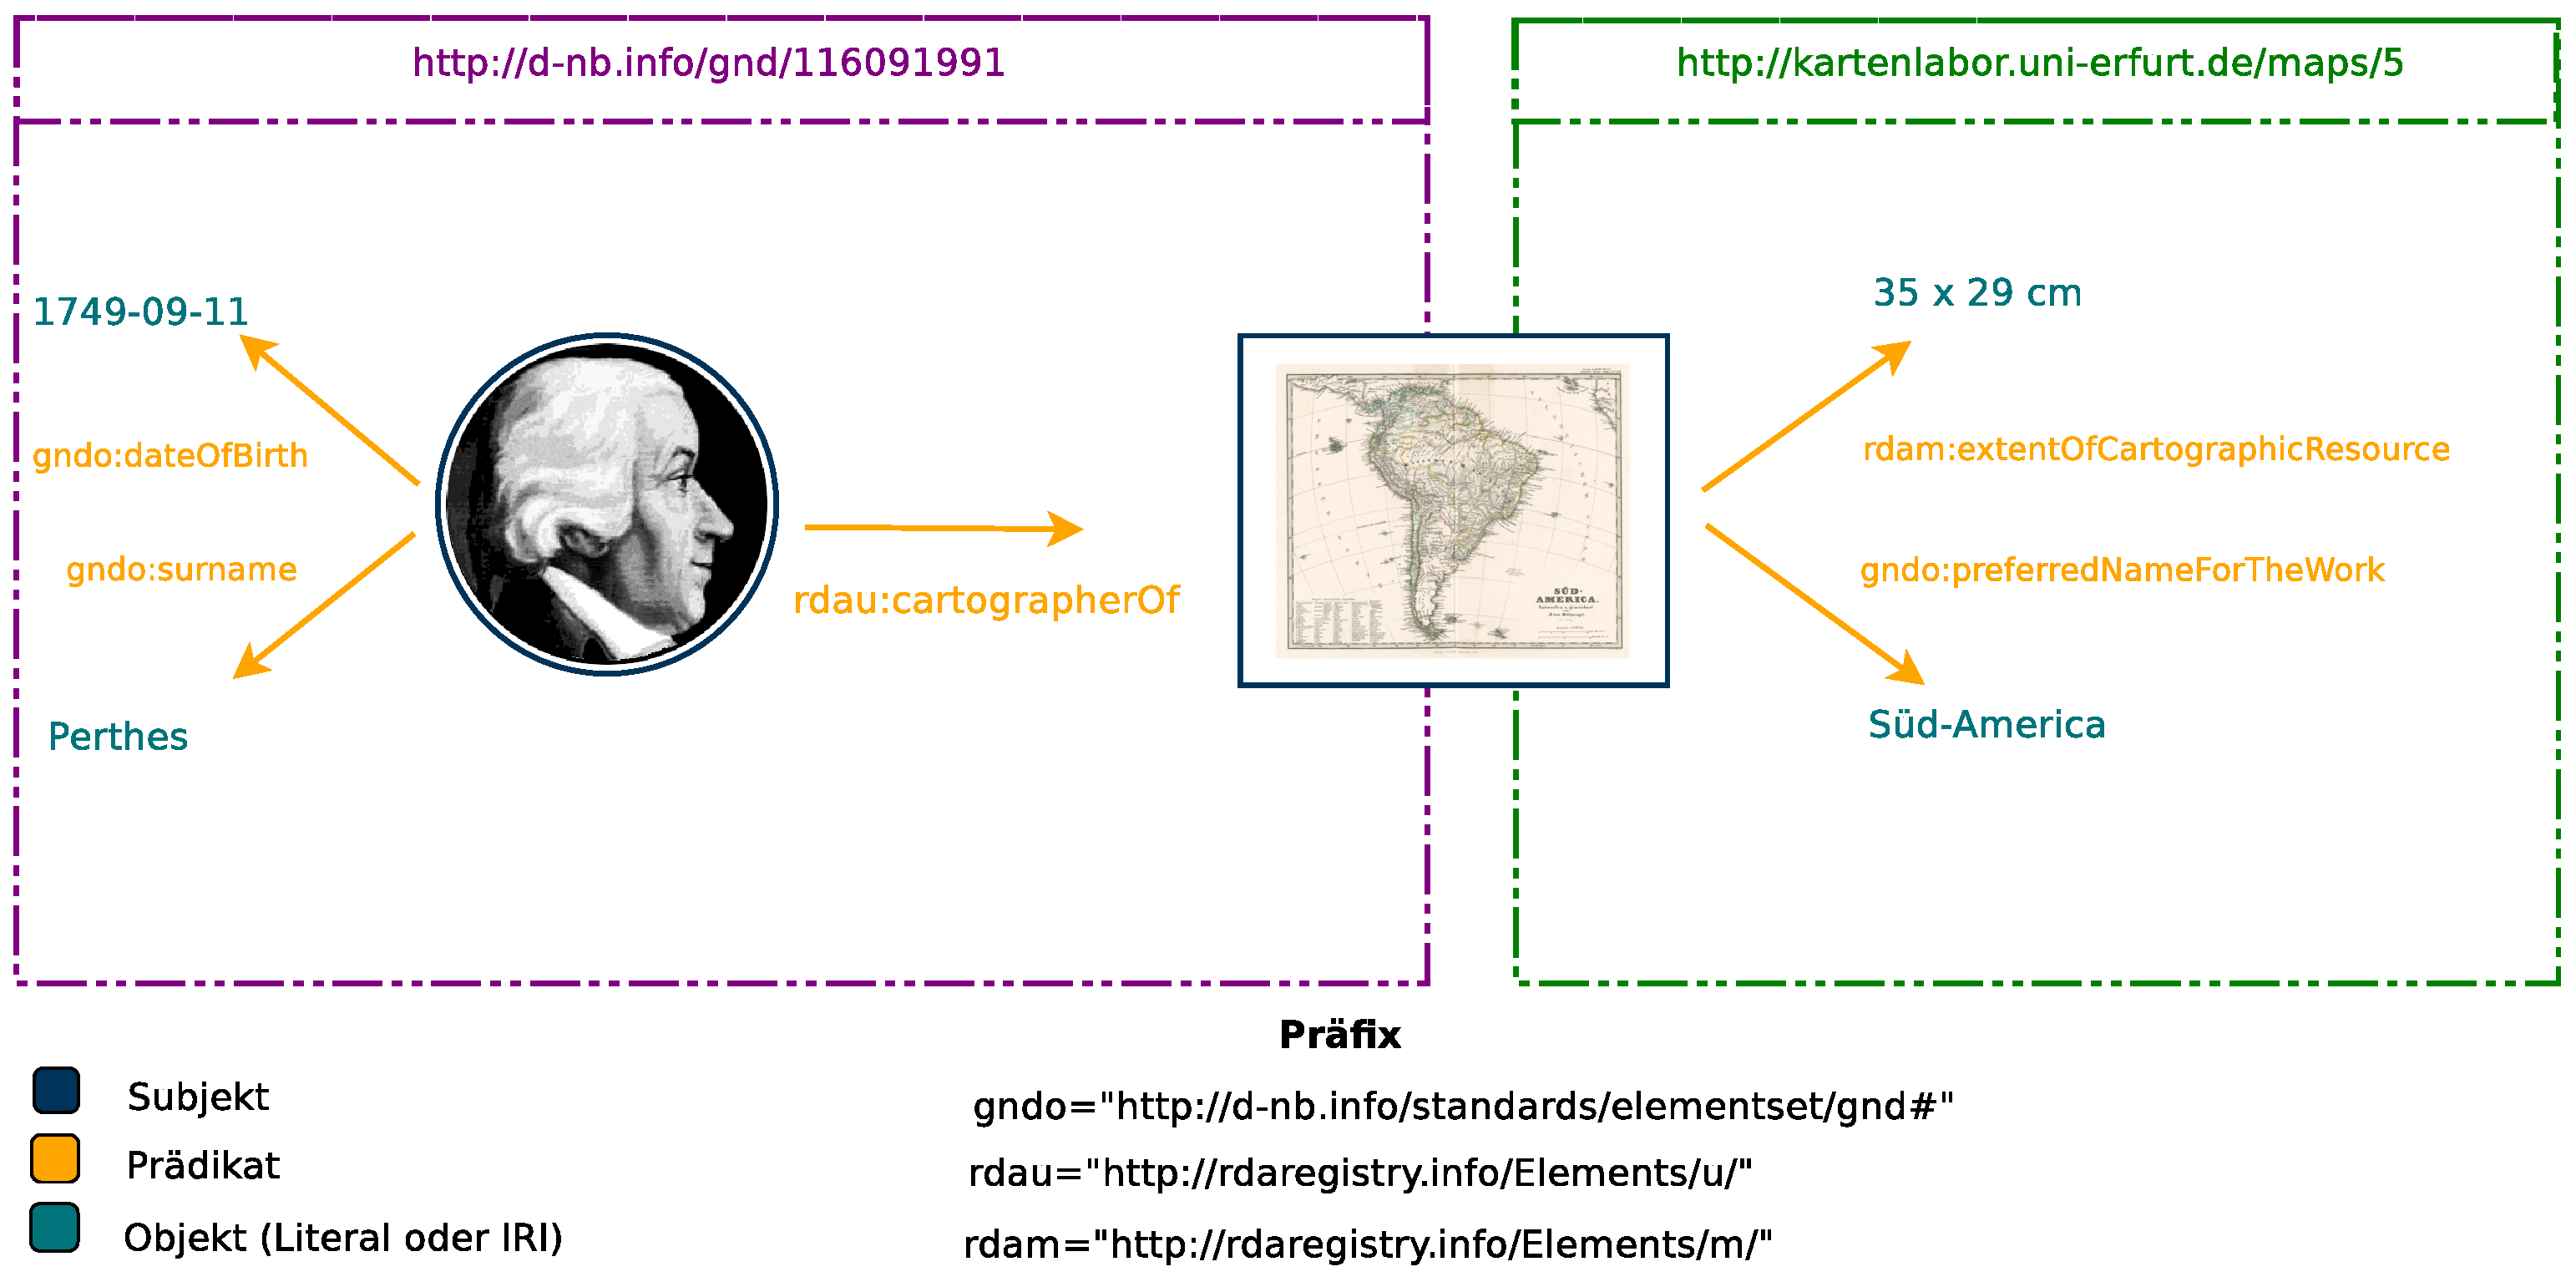
\includegraphics[width=1\linewidth]{images/rdf-intro}
	\caption[Linked Data mit RDF]{Linked Data mit RDF}
	\label{fig:rdf-intro}
\end{figure}

\subsubsection{Serialisierung}
\label{sec:serialisierung}

Mit der Freigabe von RDF 1.1 wurden vier nicht XML-basierte Serialisierungssyntaxen eingearbeitet \autocite[vgl.][Abs.~3]{Wood:14:WNR}. In dieser Arbeit werden Resource Description Framework in Attributes (RDFa) Syntax und JSON Linked Data (JSON-LD) behandelt. Die beiden Serialisierungssyntaxen ermöglichen semantische Annotation (vgl. \autoref{sec:linked-data} für Definition) in Anwendungsfeldern, wo es vorher mit klassichen RDF/XML nicht ideal war. Semantische Annotation ist nach \citeauthor[S.~405f]{reif2006semantic}, \hyphenquote{german}{den Prozess des Hinzufügens von semantischen Meta-Daten zu Dokumenten, die den Inhalt eines Dokuments in maschinen-verarbeitbarer Form beschreiben}.

RDFa macht es möglich maschinenlesbare Metadaten in Webseiten einzubinden, indem es neue HTML-Attributen für diesen Zweck festlegt. Diese \hyphenquote{german}{Anreicherung} der Metadaten einer Website führt dazu, dass Fremdsoftware in der Lage ist die Metadaten der Webseite automatisch verarbeiten zu können, und dass Suchmaschinen eine gezieltere Darstellung des Websiteinhalts für Suchergebnisse anbieten können \autocite[vgl.][Abs.~2]{Schreiber:14:RP}, wobei der letztere Punkt insbesondere dann der Fall ist, wenn die Metadaten an weit verbreitete Ontologien und Vokabulare angeglichen werden. Eine RDFa Serialisierungsmöglichkeit für das Datenmodell in \autoref{fig:html-map} wurde in \autoref{lst:rdfa} veranschaulicht.

\begin{figure}[h]
	\centering
	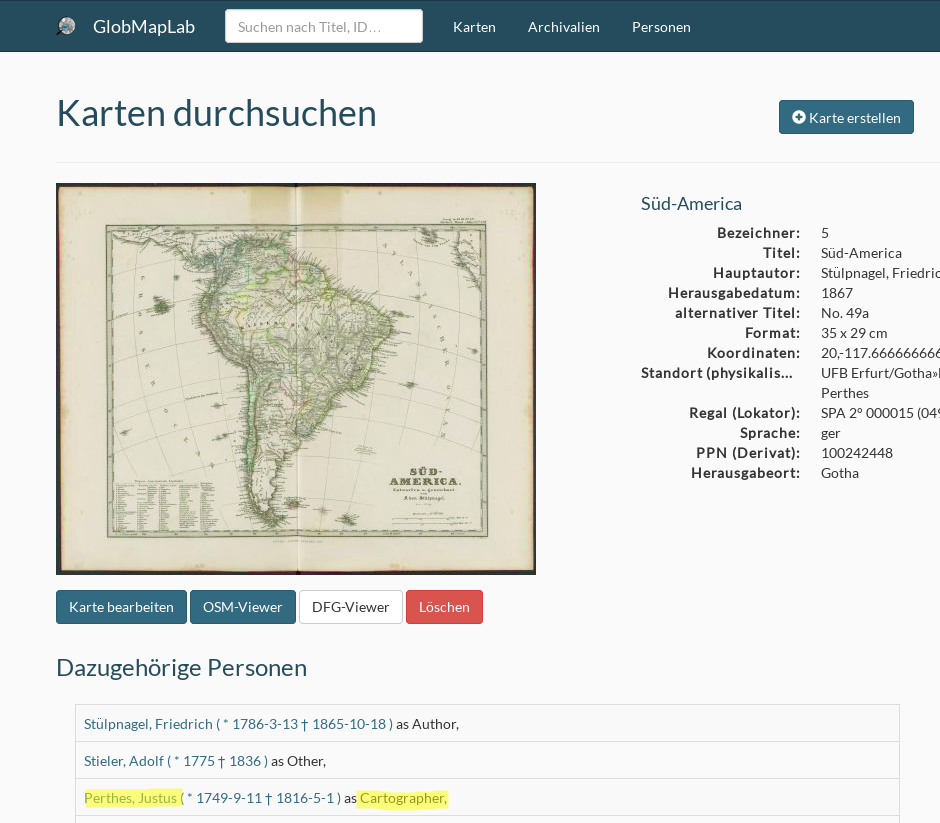
\includegraphics[width=.7\linewidth]{images/htmlmap_marked}
	\caption[Karte und Zugehörige Autoren]{Karte und Zugehörige Autoren (Screenshot vom Globmaplab Webseite)}
	\label{fig:html-map}
\end{figure}

\begin{listing}[H]
\begin{minted}[linenos,
numbersep=5pt,
frame=single,
framesep=1mm]{html}
<body prefix="gndo: http://d-nb.info/standards/elementset/gnd#
      rdau: http://rdaregistry.info/Elements/u/"
>
...
<div resource="http://kartenlabor.uni-erfurt.de/maps/5"
     typeof="http://schema.org/Map">
  <h4 property="gndo:preferredNameForTheWork">Süd-America</h4>	
  <dt>Bezeichner:</dt>
  <dd>5</dd>
  ...
</div>
...
<h3>Dazugehörige Personen</h3>
  <table>
    <tbody>
      ...
      <div resource="http://d-nb.info/gnd/116091991"
           typeof="gndo:cartographer">
        <tr property="rdau:cartographerOf" 
            resource="http://kartenlabor.uni-erfurt.de/maps/5">
          <td>
            Perthes, Justus ( * 1749-9-11 † 1816-5-1 ) 
            as Cartographer
          </td>
        </tr>
      </div>
      ...
\end{minted}
\caption{Datenmodell in RDFa}
\label{lst:rdfa}
\end{listing}

Auf die erste Zeile im \autoref{lst:rdfa} sieht man das \texttt{prefix} Attribut, das zwei Abkürzungen zu bekannten Ontologien festlegt. Das Attribut \texttt{gndo} verweist auf die Gemeinsame Normdatei (GND) Ontologie der Deutsche National Bibliothek und \texttt{rdau} auf das Resource Description \& Access (RDA) Vokabular.  Zeile 5 bis 10 bildet das HTML Definition List in der rechten Hälfte der \autoref{fig:html-map} ab. Mittels RDFa kann man zum Ausdruck bringen, dass die Definitionsliste eine Karte (\texttt{typeof="http://schema.org/Map"}) mit einem IRI Bezeichner innerhalb die Uni-Erfurt Domain und dem Namen \hyphenquote{german}{Süd-America} beschreibt. Zeile 13 bis 29 stellt die Tabelle unten in \autoref{fig:html-map} dar. Hier wird die Ressource Justus Perthes (\texttt{http://d-nb.info/gnd/116091991}) mit der Süd-America Karte verlinkt, indem er die Rolle des Kartographs übernimmt. 
\end{document}
